
%%%%%%%%%%%%%%%%%%%%%%%%%%%%%%%%%% DISSERTA��O OU TESE %%%%%%%%%%%%%%%%%%%%%%%%%%%%%%%%%%%%%%%%%
\documentclass[11pt]{report}
\usepackage{graphicx}
\usepackage[brazil]{babel}
\usepackage[latin1]{inputenc}
\usepackage{babelbib} % Esse pacote gera a bibliografia em Portugu�s. Acho que deve ser instalado algum pacote, n�o me recordo.
\usepackage{latexsym}
\usepackage{amsfonts}
\usepackage{amsthm}
\usepackage{amssymb}
\usepackage{amsfonts}
\usepackage{xypic}
\usepackage[all]{xy}

\usepackage{makeidx} %cria o �ndice remissivo
\makeindex

\vfuzz2pt % Don't report over-full v-boxes if over-edge is small
\hfuzz2pt % Don't report over-full h-boxes if over-edge is small

% TEOREMAS -------------------------------------------------------
\theoremstyle{alpha}
\newtheorem{Th}{Teorema}[section]
\newtheorem{Cor}[Th]{Corol�rio}
\newtheorem{Le}[Th]{Lema}
\newtheorem{Pro}[Th]{Proposi��o}
\theoremstyle{definition}
\newtheorem{Df}[Th]{Defini��o}
\newtheorem{Obs}[Th]{Observa��o}
\newtheorem{Dig}[Th]{Digress�o}
\newtheorem{Ex}[Th]{Exemplo}
\newtheorem{Esc}[Th]{Esc�lio}
\newtheorem{Ass}[Th]{Asser��o}

% MATEMATICA E LOGICA -------------------------------------------

\newcommand{\lan}     {\langle}
\newcommand{\ran}     {\rangle}
\newcommand{\IN}      {\mathbb{N}}
\newcommand{\A}       {\mathcal{A}}
\newcommand{\B}       {\mathcal{B}}
\newcommand{\C}       {\mathcal{C}}
\newcommand{\D}       {\mathcal{D}}
\newcommand{\F}       {\mathcal{F}}
\newcommand{\I}       {\mathcal{I}}
\newcommand{\T}       {\mathcal{T}}
\newcommand{\prem}    {\textsf{Prem}}
\newcommand{\con}     {\textsf{Con}}
\newcommand{\ta}      {\textsf{T}}
\newcommand{\ax}      {\textsf{Ax}}

\newcommand{\VAL}     {\textsc{Val}}
\newcommand{\SSB}     {{\bf SSbe}}
\newcommand{\SSO}     {{\bf SSat}}
\newcommand{\SSC}     {{\bf SSco}}
\newcommand{\SSU}     {{\bf SSmu}}

\newcommand{\two}     {{\bf 2}}
\newcommand{\twi}     {{\bf \Omega}}
\newcommand{\Rra}     {\Rrightarrow}

\newcommand{\jul}{\mathnormal{^{1}\hspace{-0,12cm}/\hspace{-0,04cm}_{2}}} 

\DeclareMathAlphabet{\mathpzc}{OT1}{pzc}{m}{it}

\begin{document}

\title{\textbf{Criptografia RSA gaussiana}}
\author{\textbf{Luis Antonio Co\^{e}lho}\vspace{2cm}\\
Relat\'{o}rio para Trabalho de Conclus\~{a}o de Curso - parte I apresentado \`{a}\\ Faculdade de Tecnologia da\\ Universidade Estadual de Campinas \vspace{2cm}\\
Orientador:
\textbf{Profa. Dra. Juliana Bueno}\vspace{2cm}\\}
 \maketitle



% ------------------------------------------------------------------------
%{
%
%%%%%%%%%%%%%%%%%%%%%%%%%%%%%%%%%%%%%%%%%%%%%%%%%%%%%DEDICAT�RIA%%%%%%%%%%%%%%%%%%%%%%%%%%%%%%%%%%%%%%%%%%%%%%%%%%%%%%%%%%%%%

\thispagestyle{empty}

\hspace{1cm} \vspace{8.5cm}


\hspace{2.83cm}\textit{\Large{Dedico este trabalho a minha turma e aminha fam\'ilia, por conta do apoio durante sua produ\c{c}\~ao. }}
                   % dedicat�ria
%}
% ------------------------------------------------------------------------
%{
%
%%%%%%%%%%%%%%%%%%%%%%%%%%%%%%%%%%%%%%%%%%%%%%%%%%%%%%%INVOCA��O%%%%%%%%%%%%%%%%%%%%%%%%%%%%%%%%%%%%%%%%%%%%%%%%%%%%%%%%%%%%%

\thispagestyle{empty}

%\vspace{20cm}

\noindent{AMO-TE TANTO, meu amor... n�o cante}\\
O humano cora��o com mais verdade...\\
Amo-te como amigo e como amante\\
Numa sempre deversa realidade.\\

 \vspace{0.5 cm}

\noindent{Amo-te afim, de um calmo amor prestante,}\\
E te amo al�m, presente na saudade.\\
Amo-te, enfim, com grande liberdade\\
Dentro da eternidade e a cada instante.\\

 \vspace{0.5 cm}

\noindent{Amo-te como um bicho, simplesmente,}\\
De um amor sem mist�rio e sem virtude\\
Com um desejo maci�o e permanente.\\

 \vspace{0.5 cm}

\noindent{E de te amar assim muito e ami�de,}\\
� que um dia em teu corpo de repente\\
Hei de morrer de amar mais do que pude.\\



(Vin�cius de Moraes, \textit{Soneto do amor total})
                   % invoca��o
%}
% ------------------------------------------------------------------------
%{
%\typeout{Acknowledgements}
%
%%%%%%%%%%%%%%%%%%%%%%%%%%%%%%%%%%%%%%%%%%AGRADECIMENTOS%%%%%%%%%%%%%%%%%%%%%%%%%%%%%%%%%%%%%%%%%%%%%%%%%%%%%%%%%%%%%%%%%%%%
\pagestyle{fancy}
%\pagestyle{fancy}
\fancyhead[C]{\textsl{Agradecimentos}}
\fancyhead[R]{7}
\fancyfoot[C]{}	


\chapter*{Agradecimentos}

\vspace{1.5cm}


\noindent Agrade�o neste trabalho primeiramente a Deus que permitiu que tudo isso acontecesse, ao longo de minha vida, e n�o somente nestes anos como universit�rio, mas que em todos os momentos � o maior mestre que algu�m pode conhecer.Agrade�o a todos os professores por me proporcionar o conhecimento n�o apenas racional, mas a manifesta��o do car�ter e afetividade da educa��o no processo de forma��o profissional, por tanto que dedicaram a mim, n�o somente por terem me ensinado, mas por terem me feito aprender. A palavra mestre, nunca far� justi�a aos professores dedicados aos quais sem nominar ter�o os meus eternos agradecimentos. Agrade�o a minha m�e Raquel, hero�na que me deu apoio, incentivo nas horas dif�ceis, de des�nimo e cansa�o e a todos que direta ou indiretamente fizeram parte da minha forma��o, o meu muito obrigado.\\
                   % agradecimentos
%}
% -----------------------------------------------------------------------
{ \typeout{Abstract}

%%%%%%%%%%%%%%%%%%%%%%%%%%%%%%%%%%%%%%%RESUMO%%%%%%%%%%%%%%%%%%%%%%%%%%%%%%%%%%%%%%%%%%%%%%%%%%%%%%%%%%%%%%%%%%%%%%%%%%%%%%%%

\thispagestyle{empty}

\hspace{1cm} \vspace{2.2cm}

\noindent {\Huge {\bf Resumo}}

\vspace{1.5cm}

\noindent O presente relat�rio exp�e o resultado parcial do projeto para TCC sobre o algoritmo de criptografia RSA gaussiano.
                    % resumo
}
% ------------------------------------------------------------------------

\setcounter{page}{1}
\tableofcontents                  % cria o �ndice

% ------------------------------------------------------------------------
{ %\typeout{Introducao}
%
%%%%%%%%%%%%%%%%%%%%%%%%%%%%%%%%%%%%%%%%%%%INTRODU��O%%%%%%%%%%%%%%%%%%%%%%%%%%%%%%%%%%%%%%%%%%%%%%%%%%%%%%%%%%%%%%%%%%%%%%%

\thispagestyle{empty}

\addcontentsline{toc}{chapter}{Introdu��o}

\chapter*{Introdu��o}


Introduza o que voc� pretende fazer no decorrer do seu trabalho.
					
\chapter {O in�cio do que n�o existe}
\label{Cap1}

Neste cap�tulo iremos escrever alguns comandos b�sicos tais como:
\begin{enumerate}
    \item Enumerar uma lista de �tens.
    \item Inserir marcador, isto �, uma bolinha preta na frente do
          par�grafo.
    \item Outros
\end{enumerate}

\section{Enumerar uma lista de axiomas}

  A seguinte enumera��o �  obviamente auto-referente,  porque o  foi
  produzido usando-se a si mesmo...

  Utilizamos  o comando
  {\bf{description}}, mas poder�amos utilizar o {\bf{enumerate}}, como
  feito acima.

\begin{description}
    \item[1.] $\vdash_{PC}\phi \rightarrow (\psi \rightarrow \phi)$
    \item[2.] $\vdash_{PC}(\phi\rightarrow(\psi\rightarrow\lambda))\rightarrow((\phi\rightarrow\psi)\rightarrow(\phi\rightarrow\lambda))$
    \item[3.] $\vdash_{PC}((\neg\phi\rightarrow\neg\psi)\rightarrow((\neg\phi\rightarrow\psi)\rightarrow\phi))$
\end{description}


\section{Como referenciar e enumerar automaticamente teoremas, lemas,  corol�rios, etc.}

Os procedimentos  abaixo s�o auto-explicativos.

 \begin{Le}\label{lema1}
  O {\bf{label}} � utilizado para dar um c�digo ao lema, teorema ou
  defini��o, para facilitar a refer�ncia no corpo do trabalho.
\end{Le}

\begin{Cor}\label{corolario2}
  Para citar um lema, teorema ou defini��o, basta digitar
  o c�digo deste, dentro do comando {\bf{ref}} .
\end{Cor}
\begin{proof}
	   � imediato a partir do lema \ref{lema1}.
\end{proof}

\begin{Le}\label{lema3}
$\vdash_{PC}(\neg\varphi\rightarrow\varphi)\rightarrow\varphi$)
\end{Le}

\begin{proof} Vejamos:\\

$
\begin{array}{lll}
1.&\vdash_{PC}((\neg\varphi\rightarrow\neg\varphi)\rightarrow((\neg\varphi\rightarrow\varphi)\rightarrow\varphi))& [\textrm{ Ax3 }]\\
2.&\vdash_{PC}(\neg\varphi \rightarrow \neg\varphi)                                                              & [\textrm{Lm \ref{lema1}}]\\
3.&\vdash_{PC}((\neg\varphi\rightarrow\varphi)\rightarrow\varphi))                                               & [\textrm{ MP em 1 e 2 }]\\

\end{array}
$
\end{proof}

Estes comandos para enumera��o  n�o precisam ser digitados, basta
voc� procurar dentro do {\bf{insert}}, na barra de ferramentas do
Winedit (se voc� estiver  trabalhando com ele) .
        
\chapter {Aritm\'{e}tica Modular}
\label{Mod}

\section{Ciclos e Restos}	
\subparagraph{
Para podermos compreender a aritm\'etica modular, precisamos come\c{c}ar entendendo o conceito de ciclicidade. Um bom exemplo deste conceito \'e o nascer do sol, que \'e um evento que ocorre sempre ap\'os um ciclo de {24} horas, assim como o dia de seu anivers\'ario ocorre uma vez a cada ciclo de um ano.
}

\section{N\'{u}meros Primos Naturais}	

\section{Per\'{i}odo e Fatora\c{c}\~{a}o}

\section{Inverso Multiplicativo}

\chapter{No caminho das nuvens}
\label{Cap2}

 Vamos neste cap�tulo nos deter a alguns detalhes tal como deixar
 o texto centralizado e como construir uma tabela.

\section{Centralizando}

Para dar destaque, por exemplo a uma equa��o no meio do texto,
deixando a mesma centralizada, basta:

$$a \wedge b \leq a $$

\noindent{digitar a f�rmula ou a equa��o entre o comando
{\bf{dolar dolar}}, como no exemplo.}

Note que para continuar o texto, foi digitado o comando
{\bf{noindent}}. Este comando serve para o programa entender que
o texto deve dar seq�encia ao texto acima, isto �, para n�o
iniciar um novo par�grafo.

\section{Tabelas}

Considere as seguintes matrizes  trivalentes onde $T$ e $T^-$ s�o
valores distinguidos:


$$
\begin{array}{|c|c|c|c|}\hline
  \wedge    & T     & T^{-}     & F \\ \hline
  T         & T^-   & T^-       & F \\ \hline
  T^-       & T^-   & T^-       & F \\ \hline
  F         & F     & F         & F \\ \hline
\end{array}
\hspace{1.5 cm}
\begin{array}{|c|c|c|c|}\hline
  \vee     & T      & T^-   & F     \\ \hline
  T        & T^-    & T^-   & T^-   \\ \hline
  T^-      & T^-    & T^-   & T^-   \\ \hline
  F        & T^-    & T^-   & F     \\ \hline
\end{array}
$$

$$
\begin{array}{|c|c|c|c|}\hline
  \rightarrow   & T     & T^-   & F     \\ \hline
  T             & T^-   & T^-   & F     \\ \hline
  T^-           & T^-   & T^-   & F     \\ \hline
  F             & T^-   & T^-   & T^-   \\ \hline
\end{array}
\hspace{1.5 cm}
\begin{array}{|c|c|c|c|c|}\hline
        & \neg_w    & \neg_s    & {\circ}_w     & {\circ}_s     \\ \hline
  T     & F         & F         & T             & T             \\ \hline
  T^-   & T^-       & F         & T             & F             \\ \hline
  F     & T         & T         & T             & T             \\ \hline
\end{array}
$$

\

As barras entre os {\bf{c}} servem para colocar as linhas
horizontais da tabela e o comando {\bf{hline}} � colocado em cada
linha que se deseja colocar a linha horizontal da tabela.

A quantidade de {\bf{c}} indicam o n�mero de colunas da tabela e
a letra {\bf{c}} indica que os dados ficar�o centralizados. Para
alinhar a direita utiliza-se a letra {\bf{r}} e para alinhar a
esquerda a letra {\bf{l}}.

Os �tens das colunas s�o separados pelo \&. Para mais detalhes
observe os exemplos.
        
\chapter{Principais resultados}
\label{Cap3}

A partir dos problemas levantados no decorrer da pesquisa sobre criptografia RSA observamos que uma parte importante do processo para criptografar uma mensagem � ter a disposi��o uma lista de n�meros primos, como um primeiro avan�o para a criptografia RSA gaussiana desenvolvemos um c�digo em linguagem Python para gerar uma lista de n�meros primos de Gauss. Resta, agora, estudar os principais resultados matem�ticos usados na criptografia RSA com o intuito de adapt�-los aos primos de Gauss.
        

\chapter{Acabando o assunto}
\label{Cap4}

\section{Diagrama}

Este � um exemplo de como construir um diagrama.

\[ \xymatrix{ A \ar[r]^f \ar[d] & D \ar[d]^{\chi_f} \\
\term \ar[r]_\top & \Omega } \]

\section{Refer�ncias}

Agora iremos fazer uma s�rie de cita��es cf. e para voc�s
aprenderem como � que se trabalha com o {\bf{bibtex}}.
        
\chapter{Cronograma}
\label{Cap5}

\begin{figure}[!htb]
	\centering
		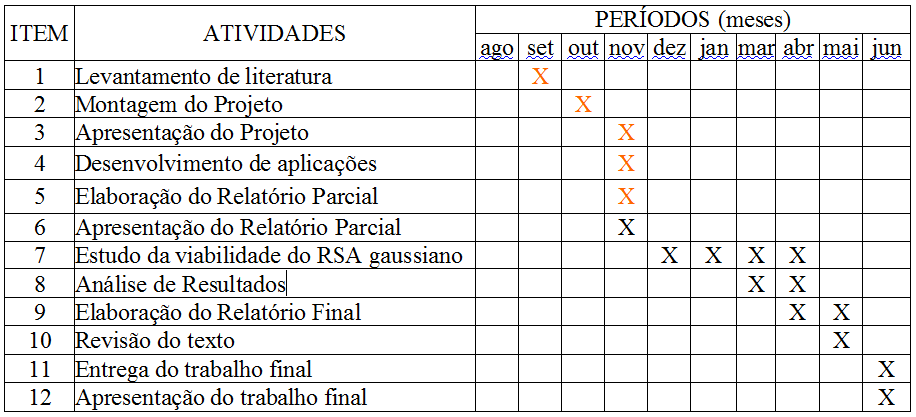
\includegraphics[scale=0.5]{figuras/cronograma.PNG}
	\caption{Cronograma com atividades realizadas e futuras}
	\label{fig:cronograma}
\end{figure}
         
\chapter{Organiza��o para conclus�o}
\label{Cap6}
\begin{enumerate}
\item{Compreender os teoremas usados na criptografia RSA.}
\item{Descrever um algoritmo para obten��o dos primos de Gauss.}
\end{enumerate}
        
%%%%%%%%%%%%%CONSIDERA��ES FINAIS%%%%%%%%%%%%%%%%%%%%%%%%%%%%%%%%%%%%%%%%%%%%%%%%%%%%%%

\pagestyle{fancy}
\fancyhead[C]{\textsl{Considera��es Finais}}
\fancyhead[R]{\thepage}
\fancyfoot[C]{}

\addcontentsline{toc}{chapter}{Considera��es Finais}

\chapter*{Considera��es Finais}

Nesta sess\~ao faremos as \'ultimas considera\c{c}\~oes sobre a viabilidade do algoritmo RSA Gaussiano. Al\'em disso vamos ver o que outros pesquisadores j\'a est\~ao concluindo em suas pesquisas.

A primeira coisa que devemos prestar aten\c{c}\~ao \'e que no decorrer desta monografia fomos capazes de descrever o funcionamento do algoritmo de criptografia RSA.

Al\'em disso demos os primeiros passos rumo a uma criptografia RSA Gaussiana, e n\~ao encontramos nada que impedisse a sua realiza\c{c}\~ao, mas como foi visto no cap\'itulo \ref{IG}, ainda precisamos da comprava\c{c}\~ao de alguns teoremas matem\'aticos importantes para a realiza\c{c}\~ao deste algoritmo. 

O material publicado por \cite{koval} e \cite{elkassar} nos leva a crer na viabiliadade do algoritmo. O que ocorre \'e que ambos possuem vis\~oes bem diferentes com rela\c{c}\~ao ao RSA Gaussiano. \cite{koval} n\~ao defende o algoritmo, pois acredita que ele n\~ao acrescenta seguran\c{c}a ao algoritmo RSA, al\'em de deix\'a-lo menos pr\'atico. Abaixo citamos o trecho onde isso \'e afirmado:

\begin{quote}
``The extension of RSA algorithm into the field of Gaussian integers [...] is viable only if real primes p congruent to 3 modulo 4 are used [...]. The extended algorithm could add security only if breaking the original RSA is not as hard as factoring. Even in this case, it is not clear whether the extended algorithm would increase security. The Gaussian integer RSA is slightly less efficient than the original, therefore the original real integer RSA is more practical.''
\end{quote}

Enquanto isso, \cite{elkassar} defende o algoritmo Gaussiano por aumentar a seguran\c{c}a comparado ao cl\'assico, como pode ser lido abaixo:

\begin{quote}

``Arithmetic needed for the RSA cryptosystem in the domains of Gaussian integers and polynomials over finite fields were modified and computational procedures were described. There are advantages for the new schemes over the classical one. First, generating the odd prime numbers in both the classical and the modified methods requires the same amount of efforts. Second, the modified method provides an extension to the range of chosen messages and the trials will be more complicated. ''

\end{quote}

Baseado nos textos de ambos podemos concluir que al\'em da realiza\c{c}\~ao de tal algoritmo, outro problema a ser investigado em um trabalho futuro consiste na an\'alise de seguran\c{c}a e complexidade do algoritmo, visto que ainda n\~ao possu\'imos uma conclus\~ao definitiva sobre isso.
        %Considera��es Finais
%
%%%%%%%%%%%%%%%%%%%%%%%%%%%AP�NDICE 1: Ipcional%%%%%%%%%%%%%%%%%%%%%%%%%%%%%%%%%%%%%%%%%%%%

\addcontentsline{toc}{chapter}{Ap�ndice 1}

\chapter*{Ap�ndice 1\\ (Opcional)}

Exemplos dos mais interessantes  manuais de latex na rede s�o os
seguintes:


P�gina sobre criptografia do IME- USP Manuais de LaTeX em
portugu�s e ingl�s, inclusive com conversoires entre LaTeX e
outros formatos:
\\
http://www.ime.eb.br/~pinho/pessoal/latex/

Manual b�sico do IFGW- UNICAMP:
\\
http://www.ifi.unicamp.br/encontro/latex-exemplo.html
         %Ap�ndice 1: Opcional

\addcontentsline{toc}{chapter}{Bibliografia} %para aparecer a  bibliografia no �ndice
%%%%%%%%%%%%%%%%%%%%%%%%%%%%%%%%%%% Comandos para gerar a bibliografia em Portugu�s %%%%%%%%%%%%%%%%%%%%%%%%

\selectbiblanguage{brazil}
%\bibliographystyle{babplain}
\bibliographystyle{babalpha}
\bibliography{Bibliografia}

%%%%%%%%%%%%%%%%%%% Caso n�o gere a bibliografia por falta de pacotes rode com os comandos abaixo e retire o pacote \usepackage{babelbib} do in�cio do documento %%%%%%%%%%%

\bibliographystyle{alpha}
\nocite{*}
%\bibliography{Bibliografia}

%%%%%%%%%%%%%%%%%%%%%%%%%%%%%%%%%%%%%%%%%%%%%%%%%%%%%%%%%%%%%%%%%%%%%%%%%%%%%%%%%%%%%%%%%%%%%%%%%%%%%%%%%%%%%
\end{document}
